\begin{savequote}[8cm]
The association of paternal and maternal chromosomes in pairs and their subsequent separation during the reducing division as indicated above may constitute the physical basis of the Mendelian law of heredity.
   \qauthor{--- \cite{Sutton1902morphology}}
\end{savequote}

\chapter{\label{ch:2-SDA} Single Cell Transcriptomics}

\minitoc

\section{Experimental Data Generation}

The experimental work in this chapter was performed by Min Jung and colleges in Don Conrad's group at the University of Washington, St Louis.

The samples generated are as follows:

\begin{itemize}
	\item 11 wild type C57BL/6 mice
	\item 3 FACS samples (primary spermatocyte , secondary spermatocyte, and spermatid) from a 12th wild type
%	\item 1 C57BL/6 mouse
	\item 1 sample of FACS sorted spermatogonial cells from 5 wild type C57BL/6 litter mates with GFP tagged Pou5f1 (B6;CBA-Tg(Pou5f1-EGFP)2Mnn/J, \cite{Szabo2002Allelespecific})
\end{itemize}

In addition to wild type mice four different mutant mice were included:
\begin{itemize}
	\item 6 Mlh3\textsuperscript{-/-} mice (B6.129-Mlh3\textsuperscript{tm1Lpkn}/J, \cite{Lipkin2002Meiotic})
	\item 2 Hormad1\textsuperscript{-/-} mice (B6;129S7-Hormad1\textsuperscript{tm1Rajk}/Mmjax, \cite{Shin2010Hormad1})
	\item 2 Cul4a\textsuperscript{-/-} mice (B6;129-Cul4a\textsuperscript{-/-}, \cite{Yin2011E3})
	\item 2 CNP eGFP BAC TRAP (knockin) C57BL/6 mice (Joseph Dougherty).
\end{itemize}

The cells were dissociated by two methods: enzymatic for the first two wild type mice and the spermatogonia, and mechanical for all other samples \cite{Lima2017Standardized,Jung2019Unified}. The cells where then encapsulated using the DropSeq protocol \cite{Macosko2015Highly} as described in \cite{Jung2019Unified}.


\section{Data Processing and QC}

The samples were sequenced on either Illumina HiSeq2500 or MiSeq. Reads were mapped to the mouse using DropSeq tools provided by Macosko lab (using STAR aligner and GRCm38 release 90).

The resulting cell-gene count matrices were merged (54,251 cells and 38,317 genes) and processed through a series of quality control and normalization steps:

Genes with a UMI count of less than 5 or being expressed in fewer than 5 cells were removed.

Cells meeting the following criteria were removed:
\begin{itemize}
\item UMI count of less than 200
\item Fewer than 100 genes expressed
\item Log UMI count more than 1 standard deviation below the mean for that experiment
\item Log number of genes expressed was more than 1 standard deviation below the mean for that experiment
\end{itemize}

A tSNE dimensionality reduction of the filtered data revealed an amorphous homogeneous group of cells with low library size, high mitochondrial gene expression and often co-expressed genes from both early and late spermatogenesis suggesting poor quality and/or doublet cells. This group of cell was therefore removed before further analysis in addition to any cells with a normalised mt-Rnr-2 expression of greater than 2 suggestive of lysed cells \cite{Ilicic2016Classification}. These filters resulted in 20,322 cells and 28,893 genes remaining.

Genes in the lower third of expression means were then removed and cells were normalized by square root transformation of total transcript counts per cell and genes were normalized to unit variance. All expression values were capped to maximum of 10. This results in a final matrix of 20,322 cells by 19,262 genes with a sparsity of 93.8\% and a median UMI count of 1,312 per cell.

SDA was then run with 50 components for 10,000 iterations.

\section{Determining an appropriate reduction dimensionality}

When performing a dimensionality reduction such as matrix factorisation we must choose the number of latent components. Too low and we may miss some real components, too high and we may find spurious components due to overfitting. One way the method can overfit is by assigning a whole component to an individual cell, which we observed (Fig \ref{fig:single_cell_component}). We found when increasing the number of components from 50 to 100 and 500 we got more of these single cell components indicating overfitting. With 50 components we had five of these components (1,4,8,14, and 46 - fig \ref{fig:SDA_diagnostics}) which we judged to be an acceptable balance between over and underfitting.

\begin{figure}[H]
	\centering
	\includegraphics[width=\textwidth]{figures/single_cell_component.pdf}
	\caption{Component 4 is represents a single cell. A) Cell scores for component 4 ordered by value. B) Gene loadings for component 4. C) Predicted expression using only component 4 vs Raw Normalised Gene Expression. Pearson's correlation is quoted (equal to correlation with the gene loadings) . All of the genes with high expression in this cell have a high gene loading in this component. D) As in C but for the cell with the second highest association. The correlation is much lower. E) As in C but using all components except 4. The correlation is less than C especially for highly expressed genes. F) As in C but using all components for the prediction.  This is the sum of C and E}
	\label{fig:single_cell_component}
\end{figure}

\section{General Properties of Inferred Components}

By inspecting the change in free energy as well as the change in fraction of gene loadings with PIP < 0.5 we can confirm that the algorithm had converged within the 10,000 iterations for which it was run \ref{fig:SDA_diagnostics}.

As expected in line with previous reports from \cite{Hore2016Tensor} the PIPs have a bimodal distribution \ref{fig:SDA_diagnostics}.

In addition the gene loadings are very sparse with 79.8\% of the gene loadings having a PIP of less than 0.5. These genes have a tight distribution of loadings around 0 with a maximum absolute loading of 0.011 and 99\% of the loadings lying within the range (-0.0033, 0.0036). Of the gene loadings with a PIP of greater than 0.5 the maximum absolute loading is 1.31 and the mean is 0.062.

Five components have outlying maximum cell scores \ref{fig:SDA_diagnostics}. These components have a single high loading in one cell and likely represent over fitting of a component to a single cell and so are not considered in further analyses \ref{fig:single_cell_component}. Two components 42, and 17 have outlying maximum gene loadings, we will later see that these components represent pachytene and spermiogenesis respectively. 

\begin{figure}[H]
	\centering
	\includegraphics[width=\textwidth]{figures/SDA_diagnostics.pdf}
	\caption{Checking convergence of SDA. A) Change in free energy is often 0 by the 10,000th iteration. B) Change in fraction of PIP <0.5 is less than 0.005\% C) Distribution of maximum scores and loadings for each component. E) Distribution of PIPs across all components, showing expected bimodal distribution.}
	\label{fig:SDA_diagnostics}
\end{figure}

\section{Low Dimensional Visualisation}

Despite reducing the dimensionality of the original dataset from 19,262 to 50 this is still too high to visualise the overall structure of the data. This can often be achieved by performing a second non-linear reduction such as tSNE or UMAP (normally PCA is the linear reduction) \cite{Maaten2008Visualizing, McInnes2018UMAPa, Becht2018Dimensionality}. We find a horseshoe like effect often found when reducing datasets with an underlying 1 dimensional structure \cite{Novembre2008Interpreting, Podani2002RESEMBLANCE}. By looking at genes with known expression patterns from the literature we can induce that in this case that the linear structure is developmental time of spermatogenesis and that the clusters in the centre are somatic cells.

To generate a pseudo-timeline we used a similar approach to that implemented in SCUBA \cite{Marco2014Bifurcation}. We iteratively fit a principal curve through the t-SNE plot with increasing degrees of freedom from 4 to 9 using the curve from the previous run as the starting point \cite{Hastie1989Principal}. Each cell was then assigned to the closest position on this curve. Somatic cells and the Hormad1 X-activated cells were excluded during pseudotime construction. Somatic cells were defined by thresholding on the cell scores of somatic components.

The order of components was determined by using a weighted mean of the pseudotime values, where the weights are the cell scores of the component. In addition only cells with an absolute cell score of greater than 2 contribute to the mean.

\begin{figure}[H]
	\centering
	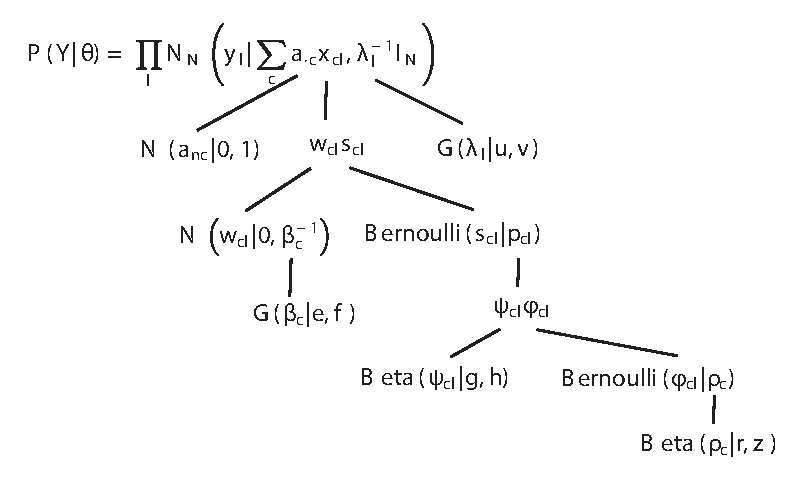
\includegraphics[width=\textwidth]{figures/SDA.pdf}
	\caption{}
	\label{fig:SDA}
\end{figure}

We can perform the same visualisation on the transposed cell scores or gene loadings to see how the components relate to each other. We find 7 major clusters of components, with hindsight these correspond to: 1) Spermatogonia, 2) Leptotene/Zygotene 3) Pachytene 4) Round Spermatid (Acrosomal) 5) Spermiogenesis 6) Somatic and 7) Somatic (Sertoli). We can see that our manual labelling of the components is consistent with the clusters.

\begin{figure}[H]
	\centering
	\includegraphics[width=\textwidth]{figures/tSNE_Components.pdf}
	\caption{A low dimensional representation of the components shows 7 clusters.}
	\label{fig:tSNE_Components}
\end{figure}



\section{Imputation}

Due to low input material and limited transcript capture efficiency the original data is very sparse. 

In the process of fitting the SDA model we have also effectively imputed the data. Multiplying out the cell scores and gene loadings matrix generates a matrix of the same dimensions as the original data but populated with the model's predicted values. Visualising these new expression vectors through pseudotime in comparison to the originals there are many fewer zero values when the gene is expressed as well as fewer outliers when it's unexpressed.

A problem with validating this imputation scheme is that we can't evaluate against the true value for each cell because we don't know the true values. Instead we partition the dataset by randomly assigning each original read to either a training or test dataset and then run SDA and imputation on the training dataset only. If the imputation is working then we should be able to predict the rankings of the gene expression in the test data.



As comparisons we either simply used the reads from the corresponding cell in the training dataset or an average over all cells. If we use the training data, we do ok for the highly expressed genes but then we run out of reads and basically guessing at random for the rest. Using an average we do better for the lower expressed genes, but of course if you take the average over all cells you may as well have done a bulk sequencing experiment. We can take the area under these curves to visualise comparative accuracy for all cells, compared to the cell-wise training data we do almost always better using the imputation, particularly well when the library size is low. Using the average we also do almost always better, and best when the cell type is not like the average as you might expect.


\section{Components}

\subsection{Telocytes}
Recently telocytes were discovered to be present in the mammalian (human) testis \parencite{Marini2018Reappraising, Kuroda2004Distribution}. We find one component (\#32) matching the known combination of markers for telocytes (Cd34 and Pdgfra positive, Kit, Pecam and Acta2/\textalpha-SMA negative) in addition to many other genes specific to this cluster (Dcn, Col1a2, Col1a2, Col3a1, Col6a1, Col4a4, Col4a1, Col1a1, Lamb1, Lama2, Lamb2, Gsn, Adamts5, Mgp) representing potential novel markers for this cell type in the testis. This component is highly enriched for the GO term "extracellular matrix organization" (p=4.3e-16, OR=10.3). Their expression pattern matches what was described as an unknown mesenchymal cell population by \cite{Green2018Comprehensive} with expression of Tcf21, Arx, Vim, and Col1A1, but not Acta2 (\textalpha-SMA), or Cyp17a1.


\subsection{Leydig Cells}
Component 40 broadly marks all Leydig cells and has high gene loadings for all the major proteins required for testosterone production including Star, Cyp11a1, Hsd3b, Cyp17a1, and Hsd17b \ref{fig:testoterone} \cite{Stojkov2013Orally} in addition to other markers of Leydig cells including Insl3 and Ptgds \parencite{Balvers1998RelaxinLike, Baker2001Expression}. This component is most highly enriched for the GO term "steroid metabolic process" (p=5.3e-23, OR=11.3)

Component 26 splits Leydig cells into two main groups, distinguished by the expression of Fabp3, Gstm1, Gsta3, and Ass1.

Component 24 is a subtype of the Fabp3 expressing C26 positive cells, which has high expression of Gstm3, Mt3, Thrsp, and Jak3, but also a number of pseudogene versions of genes that are normally expressed leydig genes: Gstm2-ps1, Gm6665 (another Gstm2 pseudogene), Fabp3-ps1, Gm8834 (Gstm3 pseudogene), Gm5096 (Bhmt pseudogene), Gm6977 (Fth1 pseudogene), Gm7049 (Me1 pseudogene).

Component 19 marks cells in both major groups and is distinguished by high expression of a group endopeptidases encoded in a 300kb locus on chromosome 7 including Klk1, Klk1b1, Klk1b21, Klk1b22, Klk1b24 and Klk1b27. Some of these genes are known to be specifically expressed in Leydig cells and may be involved in remodelling of the extracellular matrix \parencite{Sanz2013RiboTag, Matsui2000Cloning, Matsui2001Mouse, Matsui2005Characterization}.

\subsection{Sertoli Cells}

Component 37 is active in cells expressing Wipf3 (aka CR16) and Ncoa2 (aka TIF2) both of which are required for fertility and have Sertoli restricted expression \cite{Suetsugu2007Malespecific, Gehin2002Function}). In addition Nxf3 is specifically expressed in Sertoli cells but not required for spermatogenesis \cite{Zhou2011Nxf3}.

%45

%16

\subsection{Macrophages}
We find one component (\#11) representing macrophage cells. This component has high loadings for Csf1r (macrophage colony-stimulating factor receptor, aka CD115), Cd163 (macrophage scavenger receptor), Cd68, Adgre1 (aka F4/80), Itgam (aka CD11b), Mrc1, Cx3cr1, Fcgr3, and the complement genes C1qa, C1qb, and C1qc. \parencite{Mossadegh-Keller2017Developmental, Fabriek2005macrophage, Sasmono2012Generation}

Immunohistochemical staining of Adgre1 found that macrophages were present within the tubule, which is typically regarded as immune privileged partly due to the blood-testis barrier formed by sertoli cell tight junctions \parencite{Fijak2006testis}. Macrophages have previously been reported within the adluminal compartment, although always in the context of testicular defects \parencite{Frungieri2002Number, Goluza2014Macrophages}.


\subsection{Lymphocytes}
Component 3 is highly enriched for genes involved in T cell activation (p=1.4e-19, OR=7.6) and has high loadings for (T-cell) lyphocyte genes including Ptprc (aka CD45, leukocyte common antigen), Cd2 (aka T-cell surface antigen) \parencite{Murray2011Protective, Murphy2012Janeway}, Ms4a4b (high protein expression in T and NK but not B cells \cite{Xu2010MS4a4B}), and the CD3 T-cell receptor complex genes: Cd3g, Cd3d, Cd3e, Trbc2, Trac \parencite{Call2002Organizing}.


\subsection{Peritubular Myoid}
% 21??

Component 10 is active in a small number of cells, likely to be peritubular myoid cells due to co-expression of Cnn3, Edn1 (Endothelin), Myh11 (Smooth muscle myosin heavy chain), and Acta2 (Smooth muscle actin) \parencite{Mayerhofer2013Human}. The most significant GO term is "muscle tissue development" (p=8.789135e-08, OR=4.97).





\subsection{Spermatogonia}

% Spermatogonia can are the most undifferentiated germ cells in the adult body. There are a number of different types which can be categorised according to the Oakberg scheme in mice \parencite{Oakberg1971Spermatogonial}. As are the most stem cell like, which divide into Apr, Aal4, Aal be \parencite{vanPelt1990Synchronization}

Five components correspond to processes in spermatogonia. Component 31 represents undifferentiated spermatogonia expressing Zbtb16 (aka Plzf) \parencite{Buaas2004Plzf} and Foxo1 \parencite{Goertz2011Foxo1}, while component 50 splits these into two subpopulations one expressing, Gfra1 (shown to be expressed in a subset of As and required for As self renewal by acting as a co-receptor for GNDF \parencite{Meng2000Regulation,He2007Gfra1}) and Glis3 \parencite{Kang2016Transcription}, and the other Nanos3 \parencite{Suzuki2009heterogeneity}, Lin28a \parencite{Zheng2009pluripotency} and Foxf1. Component 7 likely represents A1-4 spermatogonia as they express c-Kit which is expressed in differentiated (not undifferentiated) spermatogonia \parencite{Manova1990Gonadal,Schrans-Stassen1999Differential} and is required for the A1 to Al divisions \parencite{Yoshinaga1991Role}. These cells also express Stra8 which is expressed from type A spermatogonia through to preleptotene cells in response to retinoic acid \parencite{Oulad-Abdelghani1996Characterization,Zhou2008Expressiona,Endo2015Periodic} and is required for premeiotic DNA replication \parencite{Baltus2006germ}. We find they these cells are also well marked by Plppr3, Sertad4, Met, Jade2, Nanos1, Glis1 and Glis2. Component 2 includes Ctcfl, Pou4f1, and Esx1 - likely representing intermediate and type B spermatogonia \parencite{Sleutels2012male, Budhram-Mahadeo2001closely, Maezawa2018Dynamic, Li1997Esx1, Branford1997Spx1}. Component 33 is broad component covering all the stages of spermatogonia.


\subsection{(pre)Leptotene \& Zygotene}

Component 5 includes many genes required for the creation and repair of meiotic double strand breaks. This includes Prdm9 itself; components of the meiotic cohesin complex Rad21l, Smc1b, Smc3, Stag3 and Esco2 \parencite{Rankin2015Complex}; components of the telomere tethering complex Terb1, Terb2, Spdya, and Sun1 \parencite{Ding2007SUN1, Tu2017Speedy, Wang2019meiotic}; genes involved in creating DSBs Mei1, Ccdc36 (Iho1), Spo11 partner Top6bl (Gm960), and regulator Atm \parencite{Lukaszewicz2018Control, Reinholdt2005Mei1, Robert2016TopoVIBLike, Stanzione2016Meiotic, Vrielynck2016DNA}; proteins required for the creation and processing of the ssDNA intermediates and their regulators: Mcm8, Dmc1, Rad51, Rad51ap2, Atr, Brca2, Tex15, Meilb2 (Hsf2bp), Meiob, and Spata22 \parencite{Brown2015Small, Brown2014DNA, Dai2017Meiotic, Kovalenko2006RAD51AP2, Lee2015MCM89, Martinez2016BRCA2, Pacheco2018ATR, Ribeiro2018MEIOB, Widger2018ATR, Xu2017Meiosisspecific, Yang2008Mouse, Zhang2019meiosisspecific}; class I crossover (ZMM group) proteins Shoc1 (Zip2 orthologue), Tex11 (Zip4 orthologue), Msh5, Hfm1 (Mer3 orthologue) and regulator Brip1 (FancJ) \parencite{Adelman2008ZIP4H, Guiraldelli2018SHOC1, Guiraldelli2013Mouse, Rakshambikai2013Structural, Sun2016FancJ}; as well as components of the synaptonemal complex Sycp1, Sycp2, Sycp3, Syce2, Syce3, Tex12, and Six6os1 (4930447C04Rik) \parencite{Gomez-H2016C14ORF39, Syrjanen2014molecular}.


This component is also highly enriched for GWAS hits of recombination rate in Icelandic humans \cite{Halldorsson2019Characterizing}. Of the 24 significant GWAS loci identified with confidently associated causal genes, more than half (13) rank within the top 300 genes of this component, and almost all (20) rank within the top 1300 genes (p = 5.2x10-18, OR = 77.8 [95\% CI:36.4,Inf] and p = 2.4x10-20, OR = 70.1 [95\% CI:26.9,Inf]] respectively by fisher's exact test [FET]). One of the hits, Msh4, is not ranked highly in this component (2734th out of 19262), however, it is known to function as a heterodimer with Msh5, which ranks 34th \cite{Rakshambikai2013Structural}. This highlights one of the advantages of single cell RNAseq compared to GWAS for target discovery in that it does not rely on the presence of (perhaps rare, small effect) genetic variants. In addition it directly provides a list of genes rather than SNPs affecting unknown causal genes, For example the previous GWAS had identified a SNP in the intron of Ccdc43, however our expression data strongly suggested the adjacent gene Meioc (aka C17orf104) as the causal gene (ranked 183rd vs 13,651st in component 5) in addition to the subsequent reports that Meioc is responsible for maintaining an extended meiotic prophase \cite{Abby2016Implementation, Kong2014Common, Soh2017Meioc}. 

The strong enrichment of genes involved in recombination in this component suggests other highly ranked genes of unknown function could also play key roles in this process. This proved to be the case for two such genes during the preparation of this manuscript. Firstly Ankrd31 (ranked 102nd) was found to control the number, timing, and location of double strand breaks in meiosis \cite{Boekhout2018REC114, Papanikos2018ANKRD31} and Hsf2bp (now Meilb2, ranked 194th) was found to be a master regulator of meiotic recombinases \cite{Zhang2019meiosisspecific}. One candidate, Zcwpw1, will be the subject of the second part of this thesis.


\subsection{Pachytene}

Testis specific lactate dehydrogenase Ldhc \parencite{Goldberg1963Lactic, Blanco1963Lactate, Goldberg2010LDHC}, in addition to Ldha and Ldhal6b \parencite{Wang2005Cloning}, and another glycolytic enzyme Pgam2 for which protein expression was found from pachytene onwards \parencite{Fundele1987Developmental}.

Y-box proteins are abundant in spermatocytes where they bind to and repress translation of mRNA \parencite[Reviwed in]{Kleene2016Positiondependent}. Ybx2 (aka Mys2) which was found translated from pachytene onwards \parencite{Kwon1993Proteins, Oko1996Germ} (transcribed from day 17 \& in pachytene cells \parencite{Gu1998Mammalian}) and is required for fertility \parencite{Yang2005Absence}. Ybx1 (Msy1) also has a high loading, with reported mRNA detectable by northern blot from day 15 (pachytene) \parencite{Tafuri1993mouse}. Ybx3 (aka Msy4), has a high loading and is detected as protein in mid-pachytene cells \parencite{Davies2000SequenceSpecific}] and extended expression causes infertility \parencite{Giorgini2002Translational}

Poly(A) binding proteins also bind to and regulate mRNA \parencite[reviewed in]{OZTURK2018Potential}. Pabpc1 and Pabpc2 both have high loadings in component 42 and are detectable from pachytene onwards \parencite{C.Kleene1994Developmental, Gu1995Poly, Kleene1998Mouse, Lee2000Expression, Kimura2009Characterization}. Pabpc6 also has a high loading but is understudied in comparison.

Pachytene components can be readily identified by the relative lack of loadings on the X and Y chromosomes. This is due to a process whereby when homologous partners fail to synapse they are marked by HORMAD1, HORMAD2 and BRCA1. This is followed by recruitment of ATR and the creation of $\gamma$H2AX resulting in transcriptional silencing (Meiotic Silencing of Unsynapsed Chromatin). As the X and Y chromosomes are only partially homologous they fail to fully synapse and are silenced by this processes (Meiotic Sex Chromosome Inactivation, MSCI) \parencite{Turner2007Meiotic, Turner2015Meiotic}.

We are also able to track this process through pseudotime by visualising the ratio of X to autosomal expression through pseudotime (Fig \ref{fig:MSCI}). The ratio drops sharply to close to 0 before gradually recovering, although to a level below that of the original starting ratio. It has previously been reported that some sex chromosome genes are able to escape MSCI \parencite{daCruz2016Transcriptome, Soumillon2013Cellular}. However, we were unable to detect expression of these genes during the time at which MSCI is active (Fig \ref{fig:supp_MSCI}). Many of the genes had high expression just before or after MSCI, suggesting that they were previously identified due to the low stage-resolution of the previous study. 

\begin{figure}[H]
	\centering
	\includegraphics[width=\textwidth]{figures/MSCI.pdf}
	\caption{}
	\label{fig:MSCI}
\end{figure}

\begin{figure}[H]
	\centering
	\includegraphics[width=\textwidth]{figures/MSCI_supp.pdf}
	\caption{}
	\label{fig:MSCI}
\end{figure}


In addition to MSCI we may expect to observe a lack of sex chromosome transcripts due to the lack of either an X or Y chromosome in the haploid cells post meiotic division. However, from the mitotic divisions of the spermatogonia onwards cytokinesis does not fully complete and $um$-wide cytoplasmic bridges are formed between adjacent cells such that the cytoplasm could be shared across a synctium of cells \cite{Greenbaum2011Germ}. Whilst theoretically thousands of cells could be connected in practise up to 650 connected cells have been observed \cite{Ren1991Clonal}. The extent to which mRNA sharing occurs is unknown although efficient sharing has been shown for individual genes \cite{Braun1989Genetically}. If many genes were not shared we would expect to see two populations of cells after the meiotic divisions with high and low X chromosome expression respectively. However, we observe a marginal distribution of X expression conditional on pseudotime that is unimodal - suggesting that mRNA (on the X chromosome at least) is efficiently shared.

There remains a possibility that some individual or group of genes are not shared, such as has been observed for autosomal genes in a mutant heterozygous context: the t-complex responder mutant (SmokTcr) which functions as an antidote in the poison-antidote meiotic drive system of the t-complex \cite{Veron2009Retention} and Spam1 which causes transmission ratio distortion in Robertsonian (Rb) translocation-bearing mice \cite{Martin-DeLeon2005Spam1associated}.

\subsection{Hormad1 Sex Chromosome Activation}
In addition to the pachytene components with lack of loadings on the sex chromosome we also find a component (\#39) with an \textit{excess} of sex chromosome loadings relative to the autosomes. This component is active exclusively in a subset of Hormad1 KO cells that diverge from the normal pseudotime around Zygotene stage. Hormad1 KO mice arrest at early Pachytene, once the cells diverge the pseudotimes no longer match the equivalent stage of pachytene and are perhaps considerably compressed \parencite{Shin2010Hormad1}. HORMAD1 marks unsynapsed chromosomes, so when HORAMD1 is absent ()as in the KO) it appears as though the sex chromosomes are fully synapsed and transcriptional silencing fails to occur. We find that not only does Hormad1 KO fail to silence previously expressed sex-linked genes, many previously \textit{unexpressed} sex-linked genes such as Rhox2h have high expression. Interestingly, there are also multiple autosomal genes with high loadings. This may be due to ectopic expression of sex-linked transcription factors; for example, Zfy1 and Zfy2 were previously shown to cause pachytene arrest when forcibly expressed \cite{Royo2010Evidence}. We find a very strong association between genes in this component and genes overexpressed in mice which have mutations in either Hormad1 ($p = 2.2x10^{-39}$ OR = 184) or Trip13 which is required for HORMAD1 removal from synapsed chromosomes ($p = 1.3x10^{-157}$ OR = 115) \cite{Ortega2016Surveillance, Wojtasz2009Mouse}.


\subsection{Meiotic Divisions}
Component 20 contains high loadings for cell cycle associated genes such as the cyclin Ccna1 which is expressed from late pachytene through until just after the meiotic divisions \parencite{Sweeney1996distinct} for which it is required \parencite{Liu1998Cyclin}. The cyclin Ccnb1 controlling the G2/M transition is also present, along with its activators Aurka, Bora, Plk1, and Cdc25a \parencite[Reviewed in ]{Joukov2018AuroraPLK1}. The CDK2 inhibitor Cdkn3 (aka KAP1, \parencite{Poon1995Dephosphorylation}), Rgcc (regulator of cell cyle) which is required for G2/M transition \parencite{Saigusa2007RGC32}, anaphase promoting complex activator and Cdc20 homologue Fzr1 \parencite{Holt2014APC}, and Mitotic Checkpoint Complex antagonist Mad2l1bp (p31comet) \parencite{Habu2002Identification}.

The positive and negative loadings are marginally significantly enriched for ``spindle checkpoint'' and ``chromosome segregation'' GO terms respectively (p= 0.03 \& 0.015, OR= 10.4 \& 3.7).

This component is also highly enriched for a family of proteins with a domain of unknown function (DUF622) 1700001F09Rik, Gm3453, Gm10354, Gm3149, Gm8362, Gm3127, Gm17019, Gm4181, Speer4e, Speer4b, Gm9758, Gm8232, BC061237, Gm5458, 4930572O03Rik, Gm5800, Gm7361, Gm8220 (18 out of the top 88 genes). This family of genes is rodent specific and arose from duplication of the Dlg5 gene \parencite{Church2009Lineagespecific}. Interestingly it was reported that genes of this family have similar epigenetic profiles to that of the sex chromosomes in spermatogenesis \parencite{Moretti2016Expression}. This component is also host to a second family of ampliconic genes (Ssx - Synovial Sarcoma associated, on the X chromosome), discussed in further detail below.

\subsection{Round Spermatid}
Round spermatid component 30 contains many genes associated with the acrosome, an organelle which forms a nuclear cap containing hydrolytic enzymes used in fertilization (Ito and Toshimori, 2016) (Supplementary file 3). For one high loading gene, Lrrc34, we verified by immunofluorescence that the protein is indeed localized to the acrosome of round spermatids (Figure 2B). Component 35, which is essentially concurrent to component 30 in pseudotime, is the most mysterious of all components that we detected. Dozens of protein-coding genes in this component are highly enriched in testis expression but have no known function (Supplementary file 3). This component also harbors a substantial number of genes with no apparent ortholog in humans. The existence of such a set of poorly characterized genes likely reflects the difficulty of studying postmeiotic male germ cells - which cannot be differentiated in vitro, host numerous cell-type specific processes, and express many rapidly evolving genes.

\subsection{Spermatocytes}

The spermiogenesis components 17, 18 and 34 all contain many genes known to be expressed at the latest stages of spermatogenesis, before transcriptional arrest due to replacement of histones with protamines (Sassone-Corsi, 2002) (Supplementary file 3). In addition, Abhd5 (aka CGI-58), a protein previously detected in testis lipid droplets (Wang et al., 2015), has high loadings specifically in these late components (17 and 18) and we show by immunofluorescence that it serves as an excellent marker of the residual body (Figure 2B).

\subsection{Batch Effects}

In addition to transcriptional programmes we also found components representing likely batch effects. For example component 12 has high cell loadings for Hormad1 KO cells, but these loadings are largely positive for the first two batches, and negative for the last batch. Component 22 gene loadings are highly enriched in ribosomal proteins (50 of the top 100 loadings are non pseudogene ribosomal genes - of which there are 99). However unlike ribosomal component 43, the cell scores for component 22 are associated with whether the sequencing was done on MiSeq or HiSeq Illumina machines and so this component is likely a batch effect.

Component 9 contains 41 out of 57 of the respiratory complex I, III, and IV genes (complex II is an alternative pathway) (p = 7.4x10-53, OR = 104 [95\% CI: 62.1,Inf] FET). It's not clear whether this component reflects real meiotic biology or potentially reflect cell stress induced by experimental processing (still a real biological process but not one that exists in vivo).

\section{Motif Inference}
Given there exists these groups of co-expressed genes the obvious question is what's driving this expression? One major class of transcriptional regulation is the binding of transcription factors to promoters and enhancers.

\subsection{Enrichment of Known Transcription Factor Targets}
There are some transcription factors that are known to regulate meiotic gene expression. One of these is MybA (encoded by Mybl1, \cite{Bolcun-Filas2011AMYB}) and we find that the predicted direct targets of the MybA transcription factor ()as found by ChIPseq and RNAseq of KO mice) are strongly enriched specifically in the pachytene components as expected based on known targets and expression of MybA. Other known meiotic transcription factors including Stra8 \parencite{Kojima2019Amplification}, Rfx2 \parencite{Kistler2015RFX2}, and Crem \parencite{Nantel1996Spermiogenesis} are also enriched in specific components contiguous in pseudotime and consistent with their known targets.


\subsection{\emph{De-novo} inference form promoter sequences}
Transcription factors are able to recognise specific subsets of gene promoters by sequence specific binding to DNA motifs. Hence, if transcription factors are responsible for the co-expression patterns observed, we would expect to see enrichment of these binding motifs in the promoters of the co-expressed genes. However, it is possible that there are undiscovered transcription factors and or binding motifs and so instead we inferred \textit{de novo} motifs from the promoter sequences of the top genes from each component. This resulted in 16 groups of motifs including matches to the master regulators Stra8, Mybl1, Rfx2, Crem, as well as other genes required for fertility Nrf1, Etv5, Zfp143, and Rara.

\subsection{Broad-scale patterns of TFBS occurrence over PseudoTime}
Many motifs were found from multiple components and so to gain a broader view of which components these motifs act in we computed the linear association between the gene loadings and the motif presence probability for each motif-component combination. The known master regulators showed relatively specific enrichment (e.g. Stra8 in Leptotene component \#5, Mybl1 in Pachytene component \#42, and Rfx2 in Acrosomal component \#30). Most motifs, however, have a broad pattern of enrichment in either the diploid components or the haploid components. Other mechanisms which could control the fine-scale patterns of transcription we observe are transcription factor binding at enhancers (in which we did not look for motifs given their unknown locations and gene associations), chromatin status (modulating transcription factor binding), and or differential mRNA degradation.

We discovered that many of the motifs which show similar associations through pseudotime share a common property: the presence of a CpG dinucleotide. Many of diploid motifs contain a CpG dinucleotide whereas most of the haploid motifs do not. In fact the motif with the strongest association with pseudotime is not a motif per-se but simply the count of CpGs at the promoter.

CpG islands at active promoters are usually unmethylated and methylation can cause silencing \parencite{Li2014DNA}. 

Many of the diploid CpG containing motifs have methylation sensitive transcription factors, including the non-CpG exceptions NFYA and ETV5 \parencite{Domcke2015Competition, Wang2017NRF1}. This suggests that methylation may play a role in the mechanism by which the type of transcription factor used pre and post division is switched.

There are many genes that are expressed around the time of the meiotic divisions in component 20, however one family of genes (Ssxb1, Ssxb2, Ssxb3, Ssxb5, and Ssxb6) are all highly ranked (top 150) in this component. These genes are known to contain both an SSXRD and KRAB-related domain, the same two domains which are also present in Prdm9 (the only such gene for which this is true outside the Ssx X chromosome cluster). The KRAB-related domain has been studied in the context of Prdm9 where it was found to interact with the CpG binding protein CXXC1 \parencite{Imai2017PRDM9, Parvanov2017PRDM9}. The SSXRD domain has been studied in the context of the Ssxb family, where it was found to interact with the CpG binding protein CXXC2 (aka KDM2B) \parencite{Banito2018SS18SSX}. Both CXXC1 and CXXC2, as their name suggests, are members of a protein family containing the ZF-CxxC domain which mediates recruitment to unmethylated CpG islands \parencite[reviewed in]{Long2013ZFCxxC}. CXXC1 is a component of the SETD1 methyltransferase complex that catalyses H3K4me3 at CGI promoters \parencite{Lee2005CpGbinding}. CXXC2 is a demethylase which actively removes H3K36me2 at CGI promoters in addition to recruiting polycomb repressive complex 1 which in turn catalyses H2AK119ub1 \parencite{He2008H3K36, Farcas2012KDM2B, He2013Kdm2b, Wu2013Fbxl10}. H3k27me3 has been reported to increase substantially from pachytene to the round spermatid stage, and this mark can be desposited by polycomb complex 2 \parencite{Sin2015Poised}.


  
\subsection{Novel Motifs}

Some motifs have relatively poor matches to known motifs in the HOCOMOCO database. For example one motif is most similar to the ATF1/CREM motif, but lacks the central CpG dinucleotide and has an additional CAA tail. It is known that CREM is active as an alternative isoform (tau) in late spermatogenesis, and so it is possible that the alternative motif we discovered is the true motif bound in vivo \parencite{Sassone-Corsi2000CREM}. The associations with components are much more cleanly seperated into pre and post division for the new motif, being much stronger post division, consistant with the lack of CpG compared to the database motif.

Another motif had no good motif to any motif in the HOCOMOCO database, but an excellent match to a recently discovered motif for Stra8 using ChIPseq \parencite{Kojima2019Amplification}.




\subsection{Limitations \& Extensions}
Clustering of the transcriptome with respect to meiotic stage is frustrated by promiscuous transcription~\cite{Soumillon2013Cellular} and post-transcriptional regulation. For example Prm1 (Protamine 1) and Smcp (Sperm Mitochondria-associated Cysteine-rich Protein) mRNA are stored for three and seven days respectively as free ribonucleic particles before they are translated into protein on polysomes~\cite{Cullinane2015Mechanisms, Kleene1984Translational, Kleene2004Patterns}.

%This widespread uncoupling of transcription and translation is required due to the cessation of transcription in late spermatids when the nuclear DNA is compacted. 

%However this obviously frustrates attempts to identify cell types from mRNA \emph{expression} given information on protein \emph{function}. There is also widespread promiscuous transcription in testis which increases the noise levels in an a dataset with an already low signal to noise ratio.

One important next step will be to compare our results to previously published datasets from bulk-RNAseq profiling in the testis where it is possible to perform orthogonal experiments such as immunohistochemistry in order to determine cell stages.

%  it may also be possible to assess the extent of cytoplasmic sharing through intercellular bridges in post-meiotic spermatocytes via hemizygosity of SNPs / monoallelic expression~\cite{Greenbaum2011Germ, Hoffmann2016TransposonBased}.

With the transcriptional profile of meiosis is known it may be possible to deduce the gene regulatory network by incorporating the temporal expression information with an analysis of DNA sequence motifs and prior information of known transcription factors involved in meiosis~\cite{Padovan-Merhar2013Using, Goutsias2007Computational}. Methods previously used for such purposes include ARACNE, WGCNA, iRegulon, and Boolean regulatory networks~\cite{Margolin2006Reverse, Zhang2005General, Janky2014iRegulon, Moignard2013Characterization}.

Ultimately these analyses provide hypothesis in the form of new genes involved in meiosis. These predictions could be tested using an orthogonal experimental technique for example RNA in situ hybridization to confirm cell and stage expression profiles~\cite{Moffitt2016Highperformance,Choi2016Mapping}, and or gene knockouts to confirm functional importance in meiotic processes~\cite{Jamsai2010Mouse}.
